Assuming a density $\rho_0(X), \left[\rho_0(X)\right] = \frac{g}{mm^3}$ at each point we define the total momentum
\begin{align*}
 	\vL(t) &:= \intor \rho_0(X)\vV(X,t) dX, & [\vL(t)] &= [\rho_0\vV]mm^3 = \frac{g}{mm^3}\frac{mm}{ms}mm^3 = Nms
\end{align*} 
for which we postulate the balance equation
\begin{align}
	\force(t) \stackrel{!}{=} \d{\vL}{t}(t) = \vL'(t) = \intor \rho_0(X)\d{\vV}{t}(X,t) dX = \intor \rho_0(X)\vA(X,t) dX,\label{def:bal_eq}
\end{align}
given \e{resultant forces} $\force(t)$.

\subsection{Structure of force}
We assume the forces $\force(t)$ to be composed of two different sources: Forces on the boundary and body forces.
The body forces $\vB(X,t)$ measures the force per unit reference volume ($\left[\vB(X,t)\right] = \frac{N}{mm^3} = \frac{10^{6}Pa}{mm^3} = \frac{MPa}{mm^3}$) on $X$ at time $t$.
These forces are self-weight or gravity, for example.
Further, we assume to have \e{traction vectors} $\vT(X,t,N)$ (first Piola-Kirchhoff traction vector) that indicates the force working per unit
surface area ($[\vT(X,t,N)] = \frac{N}{mm^2} = MPa$) with normal $N$ at the point $X\in\partial\Or$ at time $t$.
Then the resultant forces are given as
\begin{align}
	\force(t) &:= \intorb \vT(X,t,N)dN + \intor \vB(X,t)dX, & \left[\force(t)\right] = \left[\vL'(t)\right] &= N. \label{def:force}
\end{align}

According to \e{Cauchy's stress theorem}, we can express tractions as tensor product
\begin{align}
	\vT(X,t,N) &= \vP(X,t)N,\label{def:T}
\end{align}
where $\vP$ denotes the \e{first Piola-Kirchhoff stress tensor}, which is measured in MegaPascal, i.e. $[\vP] = MPa$.
With this we have, following Gauss integral theorem,
\begin{align}
	\intorb \vT(X,t,N)dN &= \intorb \vP(X,t)NdN = \intor \divergence\vP(X,t)dX.\label{eq:div_form_traction}
\end{align}
Using representation \eqref{eq:div_form_traction} in the force composition 
\eqref{def:force} yields the following form of the balance equation \eqref{def:bal_eq}:
\begin{align}
	\intor \rho_0(X)\d{\vV}{t}(X,t) dX &= \intor \divergence\vP(X,t) + \vB(X,t) dX
\end{align}
As this balance must also be satisfied for each subvolume $\Omega_t\subset\Or$, we actually obtain a pointwise or local form as
\begin{align}
	\rho_0(X)\d{\vV}{t}(X,t) &= \divergence\vP(X,t) + \vB(X,t) \qquad \fo X\in\Or\label{def:maineq}
\end{align}

\subsection{Stress tensor definition}
%Most generally, we consider a \e{traction} force $\vt(\vx,\vn)$ at a current point $\vx\in\Omega$ in normal direction $\vn$. 
Generally, one can deal with stress tensors expressed purely on current or reference configuration and hybrids, i.e. two-point versions.
The physically directly interpretable stress tensor is the \e{cauchy stress tensor} $\vsig(\vx,t)$ defined on the current configuration,
denoting the current stress at $\vx$ on the current unit surface orthogonal to $\vn$ at time $t$.
For solids, a description of the stresses w.r.t. the reference configuration is more practical, which is why one defines
\begin{align}
	\vP(X,t) &:= J\vsig\vF^{-T} &&\text{first Piola-Kirchhoff (stress) tensor}\\
	\vS(X,t) &:= \vF(X,t)^{-1}\vP(X,t) = J\vF^{-1}\vsig\vF^{-T} && \text{second Piola-Kirchhoff tensor} \label{def:secondpiola}
\end{align}
Loosely, $\vP(X,t)$ (as a two-point tensor) describes the stresses in the current configuration per unit (undeformed) reference area at a reference point $X$.
The second Piola-Kirchhoff tensor is purely reference-based and describes the stresses in the reference configuration
per unit (undeformed) reference area at a reference point $X$, see \cite[p. 145ff]{Bonet2008}.

Generally, prescribing the stress tensors (in one form or another) will result in different material behaviour.
Usually, this stress somehow depends on the deformation $\vF(X,t)$ and $X$ (in case of inhomogeneous material).

\subsubsection{Hyperelasticity}
In our setting we deal with \e{hyperelastic materials}, which are characterized by the fact that the current stress is only dependent on the
current configuration/deformation at times $0$ and $t$.
By the variational approach, we see that the internal virtual work conjugate of $\vP$ is $\dot{\vF}$,
which allows us to define a \e{elastic potential} or \e{stored strain energy function} as
\begin{align*}
	\Psi_F(\vF(X,t),X) &:= \intl{0}{t}\vP(X,s):\dot{\vF}(X,s)ds,\\
	[\Psi_F] &= MPa = \frac{N}{mm^2} = \frac{J}{mm^2m} = \frac{mJ}{mm^3}.
\end{align*}
which denotes the work done by the stresses (in milliJoule) per unit undeformed volume from initial to current configuration at $t$,
see \cite[p.156]{Bonet2008} or \cite[p.207]{Holzapfel2000}.
Now, by definition, we have
\begin{align}
	\dot{\Psi}_F(\vF(X,t),X) = \vP(X,t):\dot{\vF}(X,t)\label{eq:psif_dt1}
\end{align}
But considering the analytical time derivative of $\Psi_F$ also gives 
\begin{align}
	\d{\Psi_F}{t}(\vF(X,t),X) = \d{\Psi_F}{\vF}(\vF(X,t),X):\d{\vF}{t}(X,t),\label{eq:psif_dt2} 
\end{align}
leads to
\begin{align*}
	0 &= \dot{\Psi}_F(\vF(X,t),X) - \dot{\Psi}_F(\vF(X,t),X)\\
	 &= \vP(X,t):\dot{\vF}(X,t) - \d{\Psi_F}{\vF}(\vF(X,t),X):\dot{\vF}(X,t)\\
	 &= \left(\vP(X,t) - \d{\Psi_F}{\vF}(\vF(X,t),X)\right):\dot{\vF}(X,t)
\end{align*}
As this must hold for any $\vF$ (and hence $\dot{\vF}$) we obtain the relation
\begin{align}
	\vP(X,t) &= \d{\Psi_F}{\vF}(\vF(X,t),X).
\end{align}
This yields a convenient way of specifying a material stress tensor by providing a suitable $\Psi_F$.
As we will consider \e{homogeneous} material, we will omit the direct spatial dependency of $\Psi_F$ on $X$ in the following.

Further, due to the principle of material frame-indifference \cite[p.198]{Holzapfel2000}, any tensor (e.g. $\vP$)
may actually only depend on the rotation-invariant part of $\vF$, i.e. $\Psi_F$ must also be invariant under rigid body rotations.
For any fixed $X,t$ we can decompose $\vF = \vR\vU$ (\cite[p.85]{Holzapfel2000}) with a
\e{rotation} part $\vR$ with $\vR^T\vR = \vI$ and \e{stretch} part $\vU = \vU^T$.
As
\[
	\vC = \vF^T\vF = (\vR\vU)^T\vR\vU = \vU^T\vR^T\vR\vU = \vU\vU = \vU^2, 
\]
one usually defines a $\Psi_C$ depending on $\vC$ instead of $\vF$.

Omitting the $(X,t)$-arguments, consider
\begin{align}
	\vP:\dot{\vF} &= \vF\vS : \dot{\vF} = \tr((\vF\vS)^T\dot{\vF}) = \tr(\vS^T\vF^T\dot{\vF})\\
	&= \vS : (\vF^T\dot{\vF}) = \vS : \frac{1}{2}(\vF^T\dot{\vF} + \vF^T\dot{\vF})  = \vS : \frac{1}{2}(\dot{\vF}^T\vF + \vF^T\dot{\vF})\\
	&= \vS : \frac{1}{2}\dot{\vC} = \frac{1}{2}\vS : \dot{\vC}
\end{align}
We hence can define
\begin{align}
	\Psi_C(\vC(X,t)) &:= \frac{1}{2}\intl{0}{t}\vS(X,s):\dot{\vC}(X,s)ds\\
		& = \intl{0}{t}\vP(X,s):\dot{\vF}(X,s)ds = \Psi_F(\vF(X,t)),
\end{align}
which gives the same strain energy function, albeit defined using $\vC$ instead of $\vF$.
The same argument as with \eqref{eq:psif_dt1}, \eqref{eq:psif_dt2} yields
\begin{align}
	0 &= \left(\frac{1}{2}\vS(X,t) - \d{\Psi_C}{\vC}(\vC(X,t))\right):\dot{\vC}(X,t).\label{eq:secondpiolahyper}
\end{align}
As again $\vC,\dot{\vC}$ is assumed arbitrary we obtain a way to specify $\vS$ via $\Psi_C$ as
\begin{align}
	\vS(X,t) & := 2\d{\Psi_C}{\vC}(\vC(X,t)).
\end{align}
As we will stick with this perspective, we will simply use $\Psi := \Psi_C$ from now on.

\subsubsection{Incompressibility}
Further, we consider \e{incompressible} material, which is expressed by the condition 
\[
	1 = J(X,t) = \det\vF(X,t) = \sqrt{\det\vC(X,t)}\quad\fo X,t.
\]
This especially means
\begin{align}
	0 &= \d{J}{t}(X,t) = \d{}{t}\sqrt{\det\vC(X,t)}\nonumber\\
	&= \d{\sqrt{\det\vC(X,t)}}{\det\vC(X,t)}\d{\det\vC(X,t)}{\vC(X,t)}:\d{\vC}{t}(X,t)\nonumber\\
	&=\frac{1}{2}\frac{1}{\sqrt{\det\vC(X,t)}} \det(\vC(X,t))\vC(X,t)^{-1}:\dot{\vC}(X,t)\nonumber\\
	&=\frac{1}{2}\sqrt{\det\vC(X,t)}\vC(X,t)^{-1}:\dot{\vC}(X,t)\nonumber\\
	&=\frac{1}{2}J(X,t)\vC(X,t)^{-1}:\dot{\vC}(X,t).\label{def:cincompconstr}
\end{align}
Now, comparing equations \eqref{eq:secondpiolahyper} and \eqref{def:cincompconstr} we obtain
\begin{align}
	0 &= \left(\frac{1}{2}\vS(X,t) - \d{\Psi}{\vC}(\vC(X,t)) + \gamma\frac{1}{2}J(X,t)\vC(X,t)^{-1}\right):\dot{\vC}(X,t),\\
	\vS(X,t) &= 2\d{\Psi}{\vC}(\vC(X,t)) + \gamma J(X,t)\vC(X,t)^{-1},\label{def:incompressible_secondpiola}
\end{align}
where $\gamma$ is an arbitrary scalar.
In order to relate this quantity to a physical quantity, we consider the concept of hydrostatic pressure in a small detour.

\paragraph{Relation to hydrostatic pressure}
In the following we omit the $(X,t)$ (or $(x,t)$) arguments for improved readability.
The Cauchy stress tensor $\vsig$ can be split into a \e{volumetric} and \e{deviatoric} part via
\begin{align}
	\vsig &= \underbrace{\vsig - p\vI}_{=:\vsig'} + p\vI, & p &:= \frac{1}{3}\tr\vsig.
\end{align}
The resulting deviatoric part is trace-free, e.g.
\begin{align}
	\tr{\vsig'} &= \tr\left(\vsig - \frac{1}{3}(\tr\vsig)\vI\right) = \suml{i=1}{3}(\vsig_{ii} - \frac{1}{3}\tr\vsig) = \tr\vsig - \tr\vsig = 0.
\end{align}
Here, the scalar $p$ is called the \e{hydrostatic pressure}, $[p] = MPa$.
From the definition \eqref{def:secondpiola} of the second Piola-Kirchhoff stress tensor we obtain the same split for $\vS$
(omitting $X,t$ arguments for readability) via
\begin{align}
	\vS &= J\vF^{-1}\vsig\vF^{-T} = J\vF^{-1}(\vsig' + p\vI)\vF^{-T}\\
		&= J\vF^{-1}\vsig'\vF^{-T} + pJ\vF^{-1}\vF^{-T}\\
		&=: \vS' + pJ\vC^{-1}.
\end{align}
Now, $\vS$ is not necessarily trace-free anymore, but we identify the property
\begin{align}
	\vS' : \vC &= J\vF^{-1}\vsig'\vF^{-T} : \vC = J\tr\bigl(\vF^{-1}\vsig'\vF^{-T}\vC\bigr)\\
		&= J\tr\bigl(\vF^{-1}\vsig'\vF^{-T}\vF^T\vF\bigr) = J\tr\bigl(\vsig'\vF^{-T}\vF^T\vF\vF^{-1}\bigr)\\
		&= \tr\vsig' = 0.
\end{align}
With this an explicit expression for the hydrostatic pressure can be given as
\begin{align}
	\vS : \vC &= (\vS' + pJ\vC^{-1}) : \vC = \vS': \vC + pJ\vC^{-1} : \vC\\
	&= pJ\tr(\vC^{-1}\vC) = pJ\tr(\vI) = 3pJ,\label{def:hydrostaticpressure}
\end{align}
Now using \eqref{def:incompressible_secondpiola} in \eqref{def:hydrostaticpressure} gives
\begin{align}
	p &= \frac{1}{3}J^{-1}\vS : \vC\\
	  &= \frac{1}{3}J^{-1}\left[2\d{\Psi}{\vC}(\vC) + \gamma J\vC^{-1}\right] : \vC\\
	  &= \gamma + \frac{2}{3}J^{-1}\d{\Psi}{\vC}(\vC):\vC,
\end{align}
so $p$ and $\gamma$ coincide if $\d{\Psi}{\vC}(\vC):\vC = 0$.
According to \cite[p. 168]{Bonet2008}, this holds true for a modified $\Psi$ given by
\begin{align}
	\hat{\Psi}(\vC) &:= \Psi(\det(\vC)^{-\frac{1}{3}}\vC)
\end{align}
Now, we can finally write
\begin{align}
	\vS(X,t) = 2\d{\hat\Psi}{\vC}(\vC(X,t)) + p(X,t)J(X,t)\vC^{-1}(X,t).\label{def:secondpiola_pressure}
\end{align}
Note that in general
\begin{align*}
	\d{}{\vC}\det(\vC)^{-\frac{1}{3}}\vC &= -\frac{1}{3}\det(\vC)^{-\frac{4}{3}}\det\vC \vC^{-1} \vC + \det(\vC)^{-\frac{1}{3}}\\
		&=-\frac{1}{3}\det(\vC)^{-\frac{1}{3}} + \det(\vC)^{-\frac{1}{3}}\\
		&=\frac{2}{3}\det(\vC)^{-\frac{1}{3}},
\end{align*}
and hence
\begin{align}
	\d{\hat\Psi}{\vC}(\vC) = \d{\Psi}{\vC}(\det(\vC)^{-\frac{1}{3}}\vC)
	= \frac{2}{3}\det(\vC)^{-\frac{1}{3}}\d{\Psi}{\vC}(\det(\vC)^{-\frac{1}{3}}\vC) \neq \d{\Psi}{\vC}(\vC).  
\end{align}
For the case of incompressible material we have $\det\vC = 1$.
Hence $\hat{\Psi} = \Psi$ and we have the final form of $\vS$ for incompressible hyperelastic material:
\begin{align}
	\vS(X,t) = 2\d{\Psi}{\vC}(\vC(X,t)) + p(X,t)\vC^{-1}(X,t).\label{def:incompressible_secondpiola_pressure}
\end{align}

\subsubsection{(Transversely) isotropic material}
We will also consider \e{isotropic} material, which means the material response is the same, independent from any rotation or translation of
the reference domain.
In other words, the strain energy function $\Psi$ is rotation-invariant, as the definition of stress tensors via derivatives already ensures translation invariance. 
The introduction of \e{fibres} via a fibre direction $\va_0(X)\in\R^3$
in the described material leads to the extended notion of \e{transversely isotropic} material, where
the strain energy function is given as
\[
	\Psi(\vC,\va_0\otimes \va_0),
\]
where the rotation-invariance holds for both arguments.

For any tensor $\vA$ with eigenvalues $\lambda_1,\lambda_2,\lambda_3$ we have the quantities
\begin{align}
	I_1(\vA) &:= \tr\vA = \lambda_1 + \lambda_2 + \lambda_3,\label{def:I1}\\
	I_2(\vA) &:= \frac{1}{2}\left((\tr \vA)^2 - \tr\vA^2\right) = \lambda_1\lambda_2 + \lambda_1\lambda_3 + \lambda_2\lambda_3,\\
	I_3(\vA) &:= \det\vA = \lambda_1\lambda_2\lambda_3,\label{def:I3}\\
	I_4(\vA,\vv) &:= \vv\cdot\vA\vv = \vA : (\vv \otimes \vv)\label{def:I4} =: \lambda^2_{\vv},\\
	I_5(\vA,\vv) &:= \vv\cdot\vA^2\vv,\label{def:I5}
\end{align}
called \e{invariants}, as they are not changing if $\vA$ is rotated by any proper orthogonal matrix.
For \e{symmetric} $\vA$ we have the derivatives of the invariants given as
\begin{align}
	\d{I_1}{\vA}(\vA) &:= \d{\tr\vA}{\vA}(\vA) = \d{\vI:\vA}{\vA}(\vA) = \vI\\
	\d{I_2}{\vA}(\vA) &:= I_1(\vA)\vI - \vA\\
	\d{I_3}{\vA}(\vA) &:= I_3\vA^{-1}\\
	\d{I_4}{\vA}(\vA,\vv) &:= \vv \otimes \vv\label{def:dI4}\\
	\d{I_5}{\vA}(\vA,\vv) &:= \vv \otimes \vA\vv + \vv\vA \otimes \vv,
\end{align}
see e.g. \cite[p.216/p.268]{Holzapfel2000}.

Now, $\Psi$ can actually be formulated using the invariants \eqref{def:I1}-\eqref{def:I5} as
\[
	\Psi(\vC,\va_0) = \Psi(I_1(\vC),I_2(\vC),I_3(\vC),I_4(\vC,\va_0),I_5(\vC,\va_0)).
\]
for which we have
\begin{align}
	\d{\Psi}{\vC}(I_1,I_2,I_3,I_4,I_5) &=
		\d{\Psi}{I_1}\d{I_1}{\vC} + \d{\Psi}{I_2}\d{I_2}{\vC} + \d{\Psi}{I_3}\d{I_3}{\vC} + \d{\Psi}{I_4}\d{I_4}{\vC} + \d{\Psi}{I_5}\d{I_5}{\vC}\\
		&= \left(\d{\Psi}{I_1} + I_1\d{\Psi}{I_2}\right)\vI - \d{\Psi}{I_2}\vC + I_3\d{\Psi}{I_3}\vC^{-1}\\
		&\quad+ \d{\Psi}{I_4}\va_0\otimes\va_0 + \d{\Psi}{I_5}(\va_0\otimes\vA\va_0 + \va_0\vA\otimes\va_0).
\end{align}

Since we consider incompressible material, $\Psi$ will not depend on the third invariant $I_3 = \det\vC = 1$ as this is already captured in the hydrostatic pressure. 
In the following, we will specify different $\Psi(I_1,I_2,I_4,I_5)$ depending on different invariants to create an additive split as 
\begin{align}
	\vS(X,t) = p(X,t)\vC^{-1}(X,t) + \vSi(X,t) + \vSa(X,t) + \vSf(X,t) +\vSv(X,t) \label{def:S_split}
\end{align}

\subsubsection{Isotropic stress tensor $\vSi$}
Now, for the isotropic part we use
\begin{align*}
	\Psi(I_1,I_2,I_3) &= c_{10}(I_1-3) + c_{01}(I_2-3), 
\end{align*}
Initially chosen constants are (see \cite{Zheng1999})
\begin{align}
	c_{10} &= 6.352e^{-10}MPa, & c_{01} &= 3.627MPa.
\end{align}
This  gives
\begin{align}
	\vSi(X,t) &= 2(c_{10} + I_1c_{01})\vI - 2c_{01}\vC(X,t)\\
	\vPi(X,t) &= 2(c_{10} + I_1c_{01})\vF(X,t) - 2c_{01}\vF(X,t)\vC(X,t)
\end{align}

\subsubsection{Anisotropic stress tensor $\vSa$}
Further, we introduce the stretch $\la > 0$ in fibre direction $\va_0(X), \no{\va_0(X)} \equiv 1$, as
\begin{align}
	\la(X,t) &:= \sqrt{I_4(\vC(X,t),\va_0(X))} = \sqrt{\va_0(X)^T\vC(X,t)\va_0(X))}\\
	&= \sqrt{\va_0(X)^T\vF(X,t)^T\vF(X,t)\va_0(X))} = \no{\vF(X,t)\va_0(X)}\label{def:fibrestretch}
\end{align}
Now, according to \cite{Markert2005}, we employ
\begin{align}
	\Psi(\la) := \sumi \frac{b_i}{d_i}(\la^{d_i} - 1) - b_i\ln\la\label{def:markertlaw}
\end{align}
with $n=1$ summands $[b_1] = MPa, [d_1] = [-]$.
Initially chosen were 
\begin{align*}
	b_1 &= 2.756e^{-5}MPa, & d_1 &= 43.373 [-].
\end{align*}
We thus have
\begin{align}
	\d{\Psi}{\vC}(\la) &= \d{\Psi}{\la}(\la)\d{\la}{I_4}(I_4)\d{I_4}{\vC}(\vC,\va_0),\label{eq:dpsidC}
\end{align}
with
\begin{align*}
		 \d{\Psi}{\la}(\la) &= b_1\la^{d_1-1} - b_1\la^{-1} = b_1\la^{-1}(\la^{d_1} - 1),\\
		 \d{\la}{I_4}(I_4) &= \frac{1}{2\sqrt{I_4}} = \frac{1}{2\la}.
\end{align*}
With \eqref{def:dI4} and the above we get
\begin{align*}
	2\d{\Psi}{\vC}(\la) &= 2\left(b_1\la^{-1}(\la^{d_1} - 1)\right) \frac{1}{2\la}\va_0\otimes\va_0
	= \frac{b_1}{\la^2}\left(\la^{d_1} - 1\right) \va_0\otimes\va_0,
\end{align*}
leading to
\begin{align}
	\vSa(X,t) &= \frac{b_1}{\la^2(X,t)}\left(\la^{d_1}(X,t) - 1\right) \va_0(X)\otimes\va_0(X)\\
	\vPa(X,t) &= \frac{b_1}{\la^2(X,t)}\left(\la^{d_1}(X,t) - 1\right) \vF(X,t)\va_0(X)\otimes\va_0(X)
\end{align}

\paragraph{``Numerically improved'' markert law}
The energy density function \eqref{def:markertlaw} has the slight disadvantage
of leading to nonzero derivatives of the effectively applied function $\frac{b_1}{\la^2}\left(\la^{d_1} - 1\right)$ near $\lambda=1$.
As the Markert law is only applicable for $\lambda>1$, quickly increasing parameterizations (e.g. for large $b_1$ and moderate $d_1$, see Figure \ref{fig:steepmarkert})
develop discontinuous derivatives at $\lambda=1$. This is numerically problematic the stiffer the material modeled is.
\begin{figure}[!ht]
	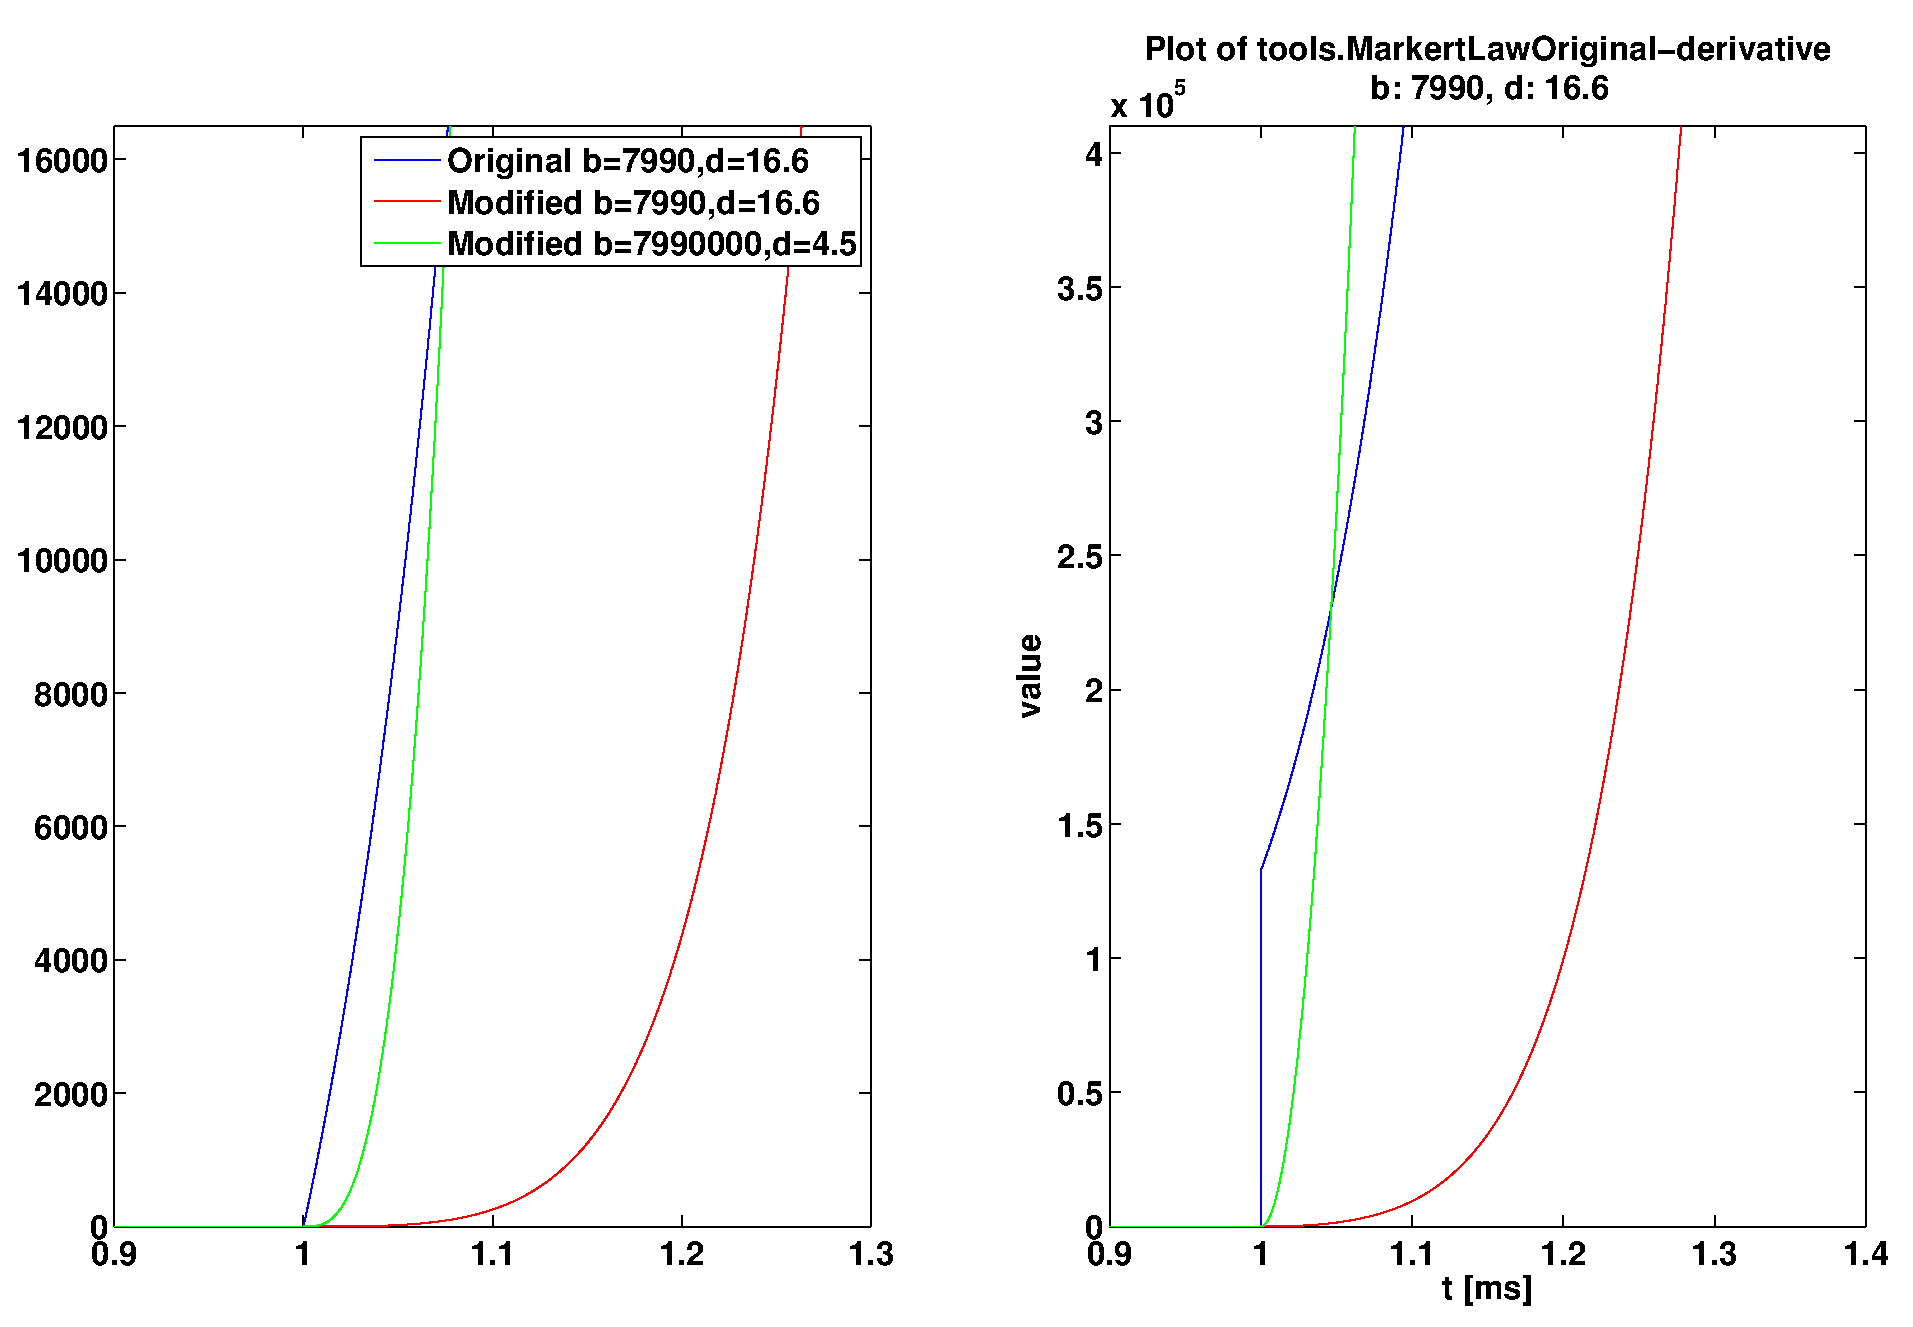
\includegraphics[width=\textwidth]{MarkertLawOriginal}
	\caption{Markert law for $b_1=7990 [MPa]$ and $d_1=16.6 [-]$ in blue. Discontinuous derivative at $\lambda=1$ with gap size $b_1d_1=132634 [MPa]$. Red shows the modified
	variant with same ``old'' parametrization and the green line is an example parameterization with similar shape}
	\label{fig:steepmarkert}
\end{figure}
A modification of the law allows to circumvent this issue by assuming the following strain energy function:
\begin{align}
	\tilde{\Psi}(\la) &:= b\left(\left(\frac{\la}{d+2}-\frac{2}{d+1}\right)\la+\frac{b}{d}\right)\la^d - \frac{b\la^2}{2} + 2b\la - b\ln\la\\
	\Psi(\la) &:= \tilde{\Psi}(\la) - \tilde{\Psi}(1)\label{def:markertlaw2}
\end{align}
For this we verify that $\Psi(1) = 0, \lim\limits_{\la\to0}\Psi(\la)=\infty$ and
\begin{align*}
	\Psi'(\la) &:= \frac{b}{\la}(\la^d-1)(\la-1)^2.
\end{align*}
Using this in \eqref{eq:dpsidC} we obtain
\begin{align*}
	\d{\Psi}{\vC}(\la) &= \frac{b}{\la^2}(\la^d-1)(\la-1)^2 =: g(\la)\\
	g'(\la) &= \frac{b(\la-1)}{\la^3}\left((d(\la-1)+2)\la^d - 2\right),
\end{align*}
for which we quickly verify that $\d{\Psi}{\vC}(1) = 0, g'(1) = 0$.

\subsubsection{Active force tensor $\vSf$}\label{sec:active_force}
We further assume to have a muscle activation $\alpha(X,t) \in [0,1]$, which is given by manual settings or motorunit models.
We then define
\begin{align}
	\Psi(\la) &:= \intl{0}{\la} p^{act}(s)ds,\nonumber\\
	p^{act}(\la) &:= p^{max}f_l(\la)f_v(\dla)\alpha(X,t),\nonumber\\
	f_l(\la) &:= \begin{cases}
		-\frac{25}{4}\left(\frac{\la}{\lfo}\right)^2 + \frac{25}{2}\frac{\la}{\lfo} - 5.25 & 0.6 \leq \frac{\la}{\lfo} \leq 1.4\\ 
		0 & \text{else}
	\end{cases} \label{def:fl},\\
	f_v(\dla) &:= ??,
\end{align}
with maximum pressure $p^{max}, [p^{max}] = MPa$.
Similar to \eqref{eq:dpsidC} we obtain
\begin{align}
	\d{\Psi}{\vC}(\la) &= \frac{p^{max}}{2\la}f_l(\la)f_v(\dla)\alpha(X,t)\va_0\otimes\va_0
\end{align}
This gives
\begin{align}
	\vSf(X,t) &= \frac{p^{max}}{\la(X,t)}f_l(\la(X,t))f_v(\dla(X,t))\alpha(X,t)\va_0(X)\otimes\va_0(X)\\
	\vPf(X,t) &= \frac{p^{max}}{\la(X,t)}f_l(\la(X,t))f_v(\dla(X,t))\alpha(X,t)\vF(X,t)\va_0(X)\otimes\va_0(X)
\end{align}

\subsubsection{Dynamic viscosity / viscous damping tensor $\vSv$/$\vPv$}
We introduce the viscous part of the stress tensor in the current configuration by defining
\begin{align}
\vPv(X,t) := \eta\,\dot{\vF}(X,t) \,,
\end{align}
where $\eta, [\eta] = MPa\ ms = \frac{g}{mm\ ms} = kP$ (kiloPoiseulle, Poiseulle = $Pa\ s$) is a parameter describing the dynamic viscosity.
%= \frac{N}{mm^2}ms = \frac{g\ mm}{mm^2 ms^2}ms = \frac{g}{mm ms} 
\\
For the second Piola-Kirchhoff tensor that means
\begin{align}
\vSv(X,t) := \eta\,\vF^{-1}\dot{\vF}(X,t) \,.
\end{align}

\subsubsection{Overall stress tensor}
Adding the different parts together as given in \eqref{def:S_split} now gives
\begin{align}
	\vS(X,t) &= p(X,t)\vC^{-1}(X,t) + 2(c_{10} + I_1c_{01})\vI - 2c_{01}\vC(X,t)\label{def:overallS}\\
			 &\quad+\Biggl[\frac{b_1}{\la^2(X,t)}\left(\la^{d_1}(X,t) - 1\right)\nonumber\\
			 &\quad+\frac{p^{max}}{\la(X,t)}f_l(\la(X,t))f_v(\dla)\alpha(X,t)\Biggr]\va_0(X)\otimes\va_0(X)\\
			 &\quad+\vSv(X,t)\nonumber\\
	g(\la,\dla,\alpha)&:= \frac{b_1}{\la^2}\left(\la^{d_1} - 1\right)
		+\frac{p^{max}}{\la}f_l(\la)f_v(\dla)\alpha\label{def:g}\\			 
	\vP(X,t) &= \vF(X,t)\vS(X,t)\label{def:completeP}\\
			 &= p(X,t)\vF^{-T}(X,t) + 2(c_{10} + I_1(\vC(X,t))c_{01})\vF(X,t) - 2c_{01}\vF(X,t)\vC(X,t)\nonumber\\
			 &\quad+g(\la(X,t),\dla(X,t),\alpha(X,t))\vF(X,t)\va_0(X)\otimes\va_0(X)+\eta\,\dot{\vF}(X,t)\nonumber
\end{align}

\subsubsection{Initial conditions}
The reference configuration is \e{stress-free}, which means that $\vP(X,t) = \vS(X,t) = 0$.
With the incompressibility conditions we also have
\begin{align*}
	\vF(X,0) &= \vC(X,0) = \vI_3, & \det(\vF(X,0)) &= 1\\
	I_1(\vC(X,0)) &= \tr(\vI_3) = 3, & I_4(\vC(X,0),\va_0) & = \vI_3 : \va_0(X)\otimes\va_0(X)\\
		\dot{\vF(X,0)}&=\vnull,&&	= \tr(\va_0(X)\otimes\va_0(X)) = \no{\va_0}^2 = 1,\\
		\la(X,0) &= 1, f_l(1) = 1, f_v(1) = 1, & \alpha(X,0) &= 0,
\end{align*}
Hence we obtain from \eqref{def:overallS}
\begin{align}
	0 &= \vS(X,0) = p(X,0)\vI + 2(c_{10} + 3c_{01})\vI - 2c_{01}\vI\\
			 &\quad+\left(\frac{b_1}{1}\left(1 - 1\right)+\frac{p^{max}}{1}1\cdot1\cdot0\right)\va_0(X)\otimes\va_0(X)
			 +\eta\vI\vnull\nonumber\\
			 & = (p(X,0) + 2c_{10} + 4c_{01})\vI\\
			 p(X,0) &= -(2c_{10} + 4c_{01})
\end{align}

% \subsubsection{Detour}
% Prescribing $\vP$ will yield the behaviour of the overall system.
% The equation $\eqref{def:T}$ also holds for values in the current configuration, i.e.
% \[
% 	\vt(x,t,n) = \vsig(x,t)n,
% \]
% where $\vsig$ is the symmetric \e{Cauchy stress tensor}.
